This chapter will show use cases showing how the simulator can be used.

\section{Use case 1}\label{sec:usecase1}
	\subsection*{2 Versus 2}
	In this first usecase, we demonstrate a simple battle between two teams, each with two regiments. For this simple battle, a $4\times4$ grid is provided by the config file, as can be seen by the Width and Height definitions. The additional standard-values and maxima-values can also be seen in the configurations file.\\
	As mentioned above, each team use the same two regiments - the only difference is the RegimentPosition, i.e. the start position of the regiments. \\
	The first regiment of PirateArchers have the following stats; The regiment consist of 10 ranged units, with 2 range, dealing 4 damage with an attackspeed of 1. They have 4 health points an can perform 1 move action per turn. Their behaviour is quite simple; if the enemy is within range, they attack the enemy. if the enemy is within 2 tiles of the regiment, the regiment retreats. If the regiment is not within range of an enemy, the regiment moves towards the nearest enemy.\\
	The other regiment consist of 10 melee warriors with 8 damage and 1 attack speed. These warriors have 8 health points and can perform 1 movement action per turn. This regiments behaviour is also quite simple; If able, they attack the enemy - otherwise they move towards the enemy and, if possible, attack the enemy.\\
	The fight was quite even, but in the end, the blue Ninjas won. Three screenshots from the battle can be seen in figure \ref{pic:case11}, \ref{pic:case12} and \ref{pic:case13}.
\begin{lstlisting}
Config

Grid BananaIsland
{
	Width = 4;
	Height = 4;
}
Rules
{
	Standards
	{
		Size = 200;
		Type = Melee;
		Range = 90;
		Damage = 2;
		Movement = 10;
		Health = 50;
		RegimentPosition = Position(0,0);
		Behaviour Agressive
		{
			Regiment enemy = SearchForEnemies(Size>0);
			Attack(enemy);
		}
	}
	Maxima
	{
		Size = 500;
		Regiments = 4;
		Range = 100;
		AttackSpeed=1;
		Damage=100;
		Movement = 20;
		Health = 1000;
	}
}
\end{lstlisting}
\begin{lstlisting}
Regiment PirateArcher
{
	Size = 10;
	Type = Ranged;
	Range = 2;
	Damage = 4;
	Health = 4;
	Movement = 1;
	AttackSpeed = 1;
	RegimentPosition = Position(4,5);
	Behaviour ArcherBehaviour
	{
		Regiment enemy = SearchForEnemies();
		if (enemy.Distance <= Range)
		{
			Attack(enemy);
			if(enemy.Distance < 2)
			{
				MoveAway(enemy);
			}
		}
		else
		{
			MoveTowards(enemy);
		}
	}
}
Regiment PirateWarrior
{
	Size = 10;
	Type = Melee;
	Damage = 8;
	Health = 4;
	Movement = 1;
	AttackSpeed = 1;
	RegimentPosition = Position(2,5);
	Behaviour WarriorBehaviour
	{
		Regiment enemy = SearchForEnemies();
		if (enemy.Distance <= Range)
		{
			Attack(enemy);
		}
		else
		{
			MoveTowards(enemy);
			Attack(enemy);
		}
	}
}
\end{lstlisting}

	\subsection*{Screenshots from use case 1}
		\begin{figure}[H]
			\center
			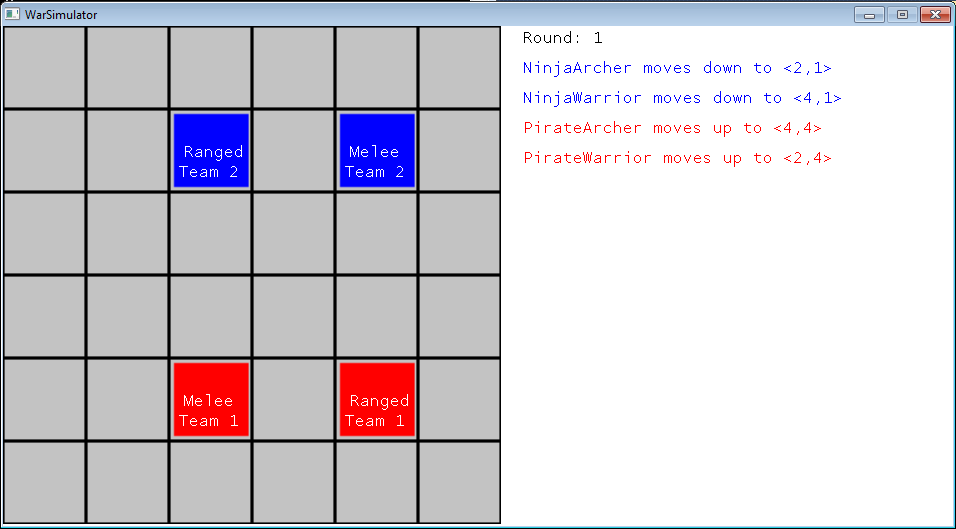
\includegraphics[scale=0.6]{rapport/7/figures/case1-1.png}
			\caption{Both teams take up an aggressive position in front of the opposing teams army.}
		\label{pic:case11}		
		\end{figure}
		\begin{figure}[H]

		\center
			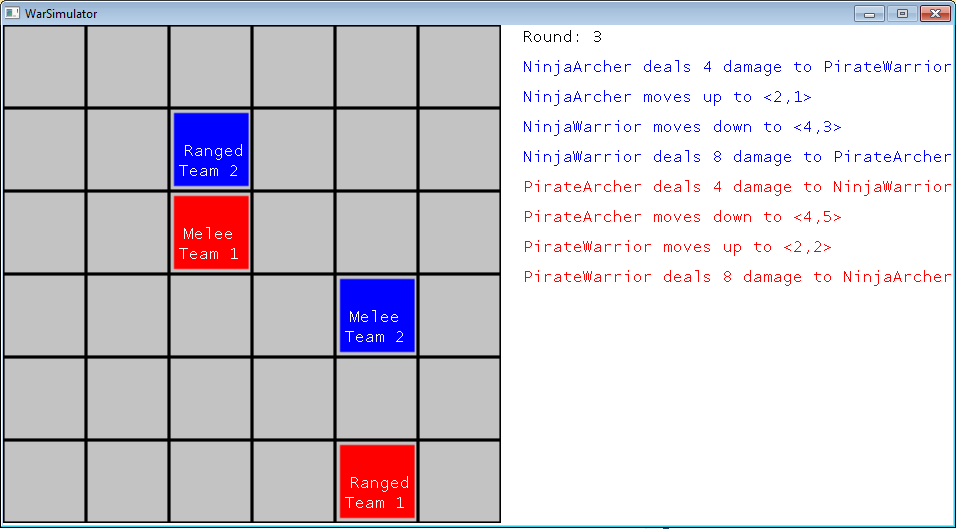
\includegraphics[scale=0.6]{rapport/7/figures/case1-2.png}
			\caption{The Warriors chase the archers, while the archers desperately try to escape}
		\label{pic:case12}
		\end{figure}
		\begin{figure}[H]
		\center
			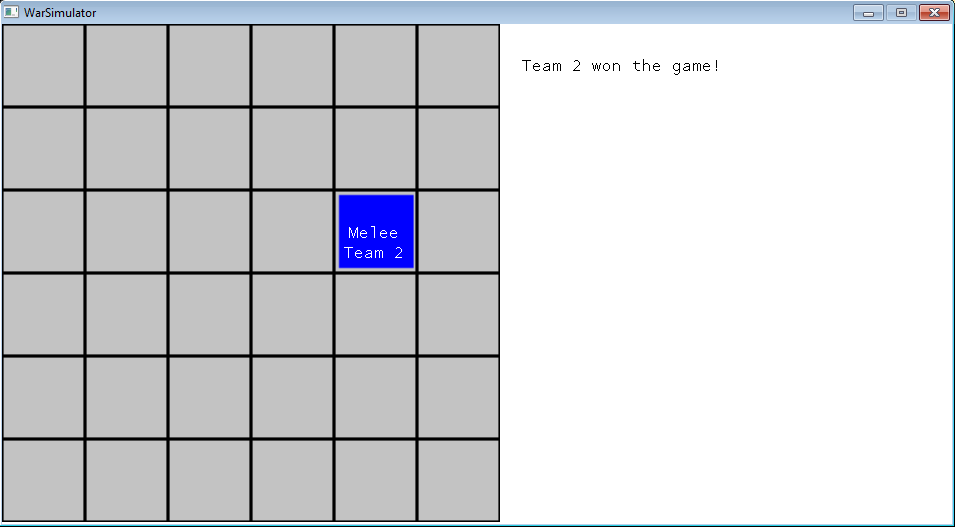
\includegraphics[scale=0.6]{rapport/7/figures/case1-3.png}
			\caption{Team 2 (The Ninjas) won!}
		\label{pic:case13}
		\end{figure}
		
\section{Use case 2}
	\subsection*{Big battle}
	Using the same regiments and config-file as seen in section \ref{sec:usecase1}, with the only alteration being the dimensions of the grid, this use case demonstrates a great battle between four opposing forces. In this scenario, the dimensions of the grid are increased to $10$. As seen on figure \ref{pic:case21} we see how all regiments engage the nearest enemies. The purple pirates seem to have taken refuge in a corner of the map. This imitates a common strategy - let the enemies fight amongst themselves, and then swoop in for the killing blow. This is also illustrated very well in figure \ref{pic:case22}, where the red, blue and green teams are at each others throat, while the purple pirates have yet to land a single strike. In figure \ref{pic:case23} we see the result of the purple pirates patience - their team won, and two regiments survived!
	
	\subsection*{Screenshots from use case 2}
		\begin{figure}[H]
			\center
			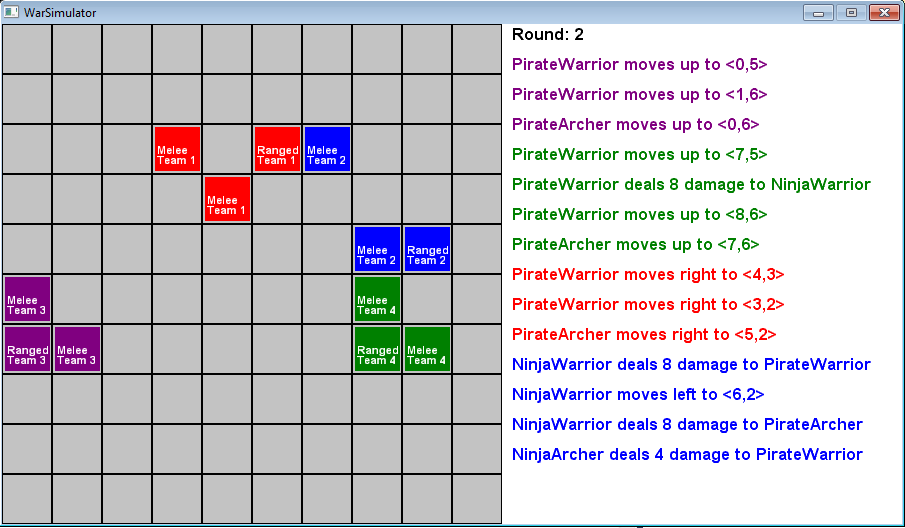
\includegraphics[scale=0.6]{rapport/7/figures/case2-1.png}
			\caption{The battle begins}
		\label{pic:case21}
		\end{figure}
		\begin{figure}[H]
		\center
			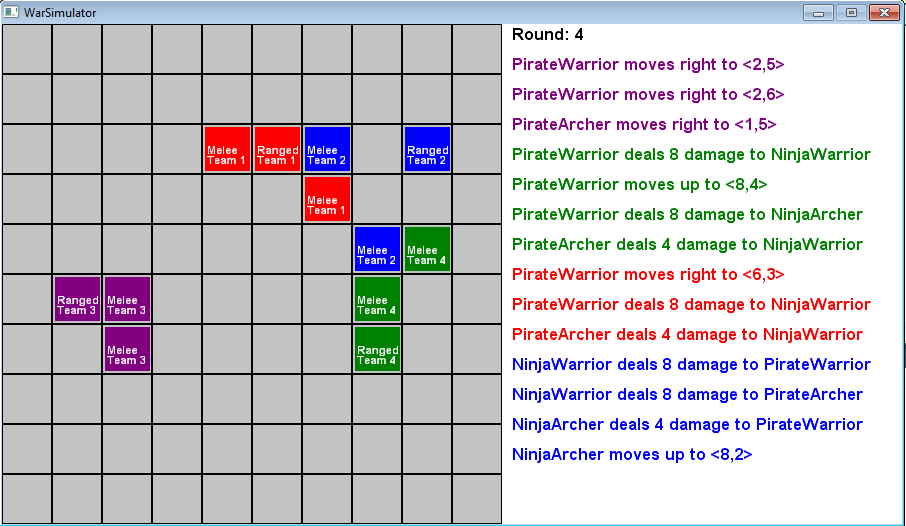
\includegraphics[scale=0.6]{rapport/7/figures/case2-2.png}
			\caption{The Purple Pirates are passive}
		\label{pic:case22}
		\end{figure}
		\begin{figure}[H]

		\center
			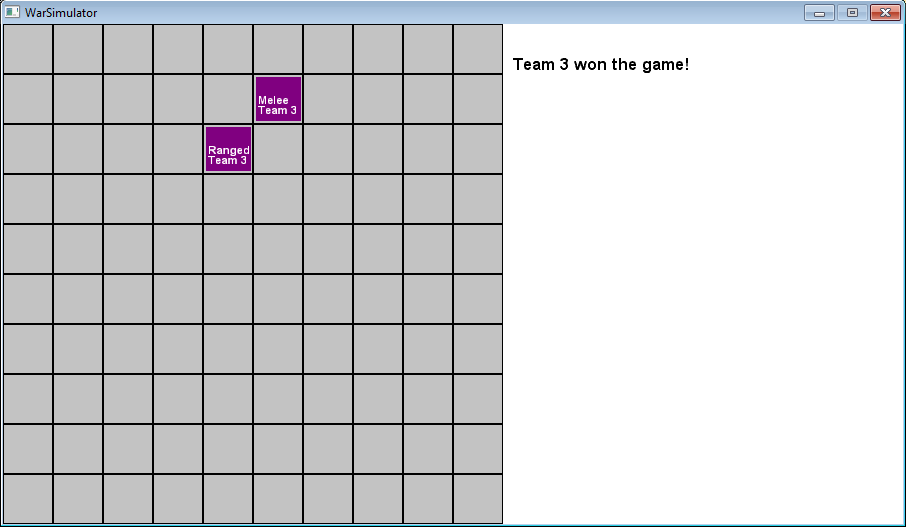
\includegraphics[scale=0.6]{rapport/7/figures/case2-3.png}
			\caption{The Purple Pirates won!}
			\label{pic:case23}
		\end{figure}
	
\section{Usecase 3}
In this usecase, we will explore the scripts of an experienced scripter versus an inexperienced scripter. The experienced scripter wrote Team 1 and the inexperienced scripter wrote Team2. The purpose of the use case is to show that the better scripter will win. \\
Team 2 consist of one slow, but dangerous melee regiment called KlamBymilits. The scriptwriter behind team 2 in convinced this regiments high damage will make it possible for him to take out both of the opponents regiments. The regiment's behaviour is extremely simple - attack any nearby enemies, and if no enemies are within range, start moving towards the enemy. \\
The scripter behind team 1 has two regiment of archers with considerably less {\it Health}. These regiments are required to use their speed and positions to defeat their enemy. The archers will spawn on each side of the enemy regiment. The behaviour of the archer regiments is designed to take advantage of the slow movement and simple tactic of the enemy. When the distance between one archer regiment and the enemy, is less than the distance between the enemy and the other archer, the archer regiment moves away from the enemy regiment. If the distance is greater, than the distance between the enemy and the friendly archer regiment, the archer regiment attacks and moves towards the enemy. \\
The result is quite spectacular - the archers successfully kite the enemy regiment in circles, and win without taking any damage.
\begin{lstlisting}
Team Team1

Regiment Archers1
{
	Size = 50;
	Range = 10;
	Damage = 10;
	Movement = 5;
	AttackSpeed = 2;
	Health = 20;
	Type = Ranged;
	RegimentPosition = Position(5,5);
Behaviour HitnRun
{
	Regiment enemy = SearchForEnemies();
	Regiment friend = SearchForFriends();
	if(enemy.Distance < (friend.Distance-enemy.Distance))
	{
		MoveAway(enemy);
		MoveAway(enemy);
	}
	else
	{
		if(enemy.Distance < Range)
		{
			Attack(enemy);
		}
		else
		{
			MoveTowards(enemy);
			MoveTowards(enemy);
		}
	}
	Attack(enemy);
}
}


Regiment Archers2
{
	Size = 50;
	Range = 10;
	Damage = 10;
	Movement = 5;
	AttackSpeed = 2;
	Health = 20;
	Type = Ranged;
	RegimentPosition = Position(15,15);
Behaviour HitnRun
{
	Regiment enemy = SearchForEnemies();
	Regiment friend = SearchForFriends();
	if(enemy.Distance < (friend.Distance-enemy.Distance))
	{
		MoveAway(enemy);
		MoveAway(enemy);
	}
	else
	{
		if(enemy.Distance < Range)
		{
			Attack(enemy);
		}
		else
		{
			MoveTowards(enemy);
			MoveTowards(enemy);
			MoveTowards(enemy);
		}
	}
	Attack(enemy);
}

}
\end{lstlisting}

\begin{lstlisting}
Team Team2

Regiment KlamBymilits
{
	Size = 20;
	Damage = 20;
	Type = Melee;
	Health = 50;
	Movement = 2;
	AttackSpeed = 1;
	RegimentPosition = Position(10,10);
Behaviour StupidBehaviour
{
	Regiment enemy = SearchForEnemies();
	if (enemy.Distance > 1)
	{
		MoveTowards(enemy);
	}
	else
	{
		Attack(enemy);
	}
}
}
\end{lstlisting}

	\subsection*{Screenshots from use case 3}
		\begin{figure}[H]
			\center
			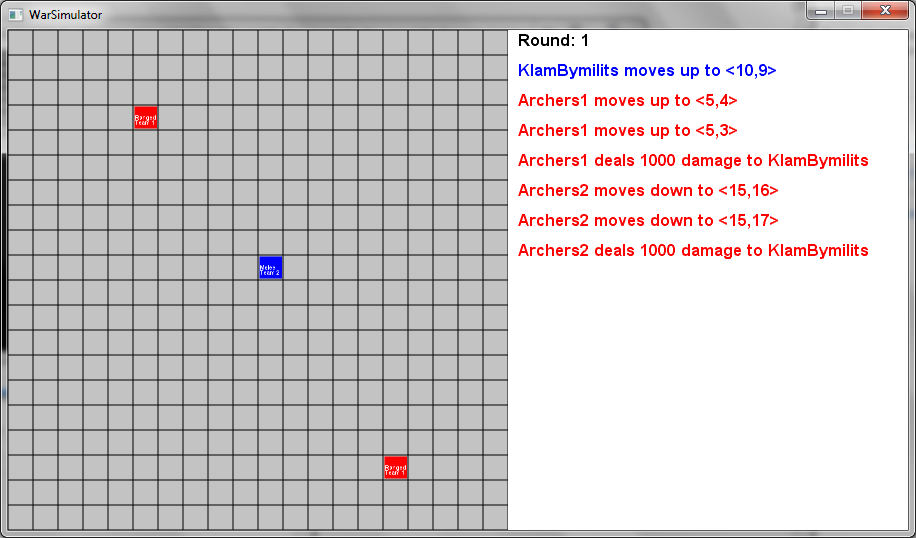
\includegraphics[scale=0.6]{rapport/7/figures/case3-1.png}
			\caption{The battle begins.}
		\label{pic:case31}
		\end{figure}
		\begin{figure}[H]
		\center
			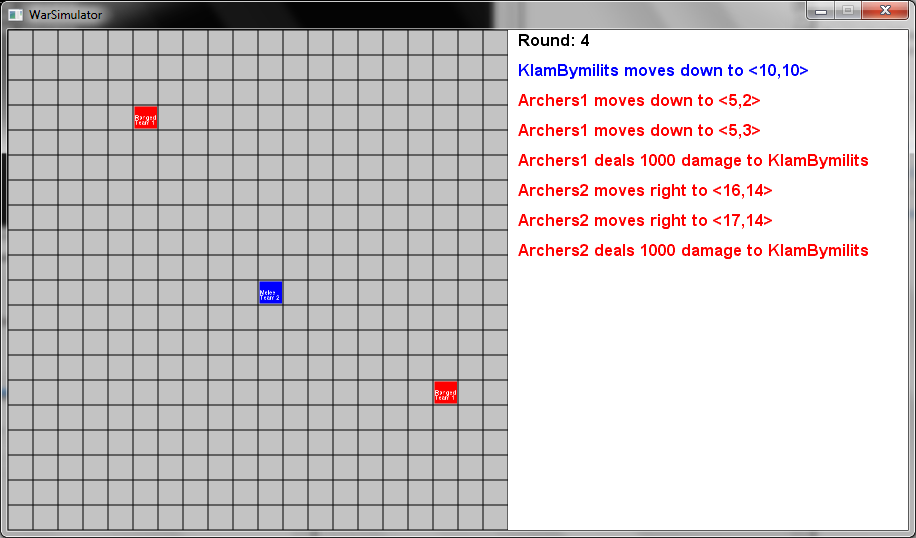
\includegraphics[scale=0.6]{rapport/7/figures/case3-2.png}
			\caption{The blue team is hesitant to attack either of the red archers.}
		\label{pic:case32}
		\end{figure}
		\begin{figure}[H]
		\center
			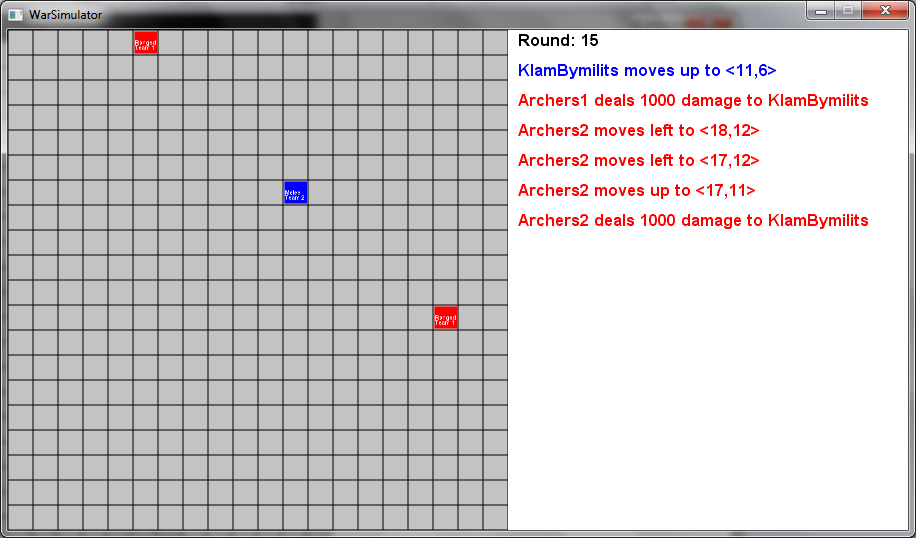
\includegraphics[scale=0.6]{rapport/7/figures/case3-3.png}
			\caption{Even after 15 rounds, the blue team is only a little better off.}
		\label{pic:case33}
		\end{figure}